\documentclass[review,3p]{elsarticle}

\usepackage{lineno,hyperref}
\modulolinenumbers[5]
\usepackage{subcaption}             % used in subtable
\usepackage{amsmath,amsfonts,amsthm}            % for subequations

\usepackage{mathtools,amssymb}          % for \leqslant
\newcommand{\ddn}[2]{\frac{\mathrm{d}}{\mathrm{d}#1}#2}
\newcommand{\ddt}{\frac{\mathrm{d}}{\mathrm{d}t}}


\usepackage{upgreek}
\usepackage[dvipsnames]{xcolor}
\usepackage{soul}
\usepackage{multirow}

\usepackage{array}
\newcolumntype{C}[1]{>{\centering\let\newline\\\arraybackslash\hspace{0pt}}m{#1}} 
\newcolumntype{L}[1]{>{\raggedright\let\newline\\\arraybackslash\hspace{0pt}}m{#1}} 
\newcolumntype{R}[1]{>{\raggedleft\let\newline\\\arraybackslash\hspace{0pt}}m{#1}} 

\usepackage{booktabs}       % http://ctan.org/pkg/booktabs

\newcommand{\tabitem}{~~\llap{\textbullet}~~}           % for items inside a table
\usepackage{makecell}       % used inside a table
\usepackage{pbox}           % for weak form 3
\usepackage{empheq}
\newcommand*\widefbox[1]{\fbox{\hspace{2em}#1\hspace{2em}}}


\usepackage{colortbl}
\usepackage{esvect}
\usepackage{spreadtab}
\usepackage{numprint}
\usepackage{xstring}
\renewcommand*{\thefootnote}{\fnsymbol{footnote}}
\usepackage[symbol]{footmisc}

\usepackage{siunitx}

\makeatletter       % for rom in deal.ii symbol
\newcommand*{\rom}[1]{\expandafter\@slowromancap\romannumeral #1@}
\makeatother

\usepackage{enumitem}

\usepackage{cleveref}
\crefformat{section}{\S#2#1#3} % see manual of cleveref, section 8.2.1
\crefformat{subsection}{\S#2#1#3}
\crefformat{subsubsection}{\S#2#1#3}

\captionsetup[figure]{labelfont={bf},name={Fig.},labelsep=period}
% \captionsetup[table]{labelfont={bf},name={Table},labelsep=space}

\usepackage[labelformat=simple]{subcaption}	        	% order of subfigure with brackets
\renewcommand\thesubfigure{(\alph{subfigure})}
\renewcommand\thesubtable{(\alph{subtable})}


\usepackage{graphicx}
\usepackage{wrapfig}
\usepackage{lipsum}

\usepackage{pgfplots}       % for tikzpicture
\pgfplotsset{compat=1.7}

\pdfsuppresswarningpagegroup=1      % eliminate warning 'multiple pdfs with page group included in a single page'

\usepackage[ruled,linesnumbered]{algorithm2e}		% for algorithm


\begin{document}

\section{Influence of d(x) and r(x) on the offset of the round-off error}         \label{discretization_error_bench_pois_diff_Helm}

% \texorpdfstring{$\alpha_{\rm R}$}{alpha_{rm R}}

We investigate the benchmark Poisson equation.
We consider $\|d\|_2$ of order 1\cite{chernetsky2010effect}.
If not stated otherwise, $P_2$ elements are used for the standard FEM, and $P_4/P_3^{\rm disc}$ elements are used for the mixed FEM.

%\subsection{\texorpdfstring{p=$e^{-(x-0.5)^2}$}{p=e^{-(x-0.5)^2}}}			\label{p_exp_2_diff_2_Helm}
% \subsection{Influence of d(x) when}

\subsection{d=1+0.5\texorpdfstring{$\sin$(cx)}{sin(cx)}, r=0}            \label{p_exp_d_1plus0p5sincx_r_0}

For $c$ being 1, 10 and 100, shapes of $d$ are shown in Fig.~\ref{shape_1_plus_sincx}, and $\|d\|_2$ are 1.23, 1.14 and 1.06, respectively. 
The analytical order of convergence can be reached within a number of $h$-refinements, and $\alpha_{\rm R}$ are shown in Fig.~\ref{alpha_R_benchmark_Pois2diff2Helm}, which are independent of $d$.

 \begin{figure}[!ht]
 \centering
     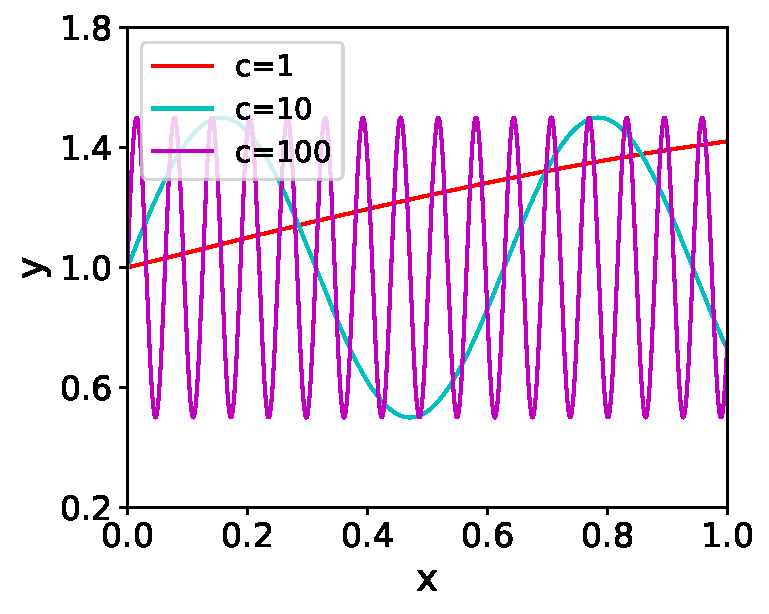
\includegraphics[width=0.4\linewidth]{py_var_1_plus_sincx.pdf}
     \caption{Shape of $d=1+0.5\sin(cx)$ for $c$ being 1, 10, 100.}
     \label{shape_1_plus_sincx}
 \end{figure}
 
\subsection{d=1+0.5\texorpdfstring{$\sin$(x)}{sin(x)}, r(x) = c}

Here, $c$ is chosen to be 1, 10 and 100. 
It is found that both the truncation error $E_{\rm T}$ and round-off error $E_{\rm R}$ are independent of $c$.
 

\begin{figure}[!ht]
\hspace{0.0cm}
\begin{subfigure}[b]{0.35\textwidth}
\scalebox{0.85}{
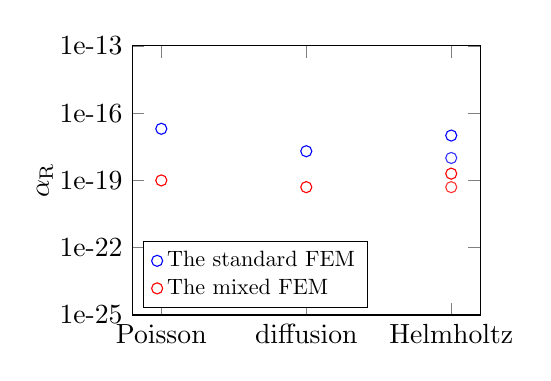
\begin{tikzpicture} 
\begin{axis}
[
    ymode=log,    
    ymin=1e-25,
    ymax=1e-13,
    ytick={1e-25, 1e-22, 1e-19, 1e-16, 1e-13},
    yticklabels={1e-25, 1e-22, 1e-19, 1e-16, 1e-13},      
    legend style={nodes={scale=0.8},at={(0.03,0.15)},anchor=west},
    legend cell align={left},
    height=5cm,
    width=6cm,
    ylabel={$\alpha_{\rm R}$},
    ylabel style={at={(-0.2,0.5)}},    
    xtick={0,1,2,3,4},
    xticklabels={Poisson, diffusion, Helmholtz}
]
\addplot[blue,mark=o, only marks,mark options={color=blue,fill=blue}] coordinates {(0,2.0e-17) (1,2.0e-18) (2,1.0e-17)};	% SM
\addplot[red,mark=o, only marks,mark options={color=red,fill=red}] coordinates {(0,1.0e-19) (1,5.0e-20) (2,2.0e-19)};		% MM


\addplot[blue,mark=o, only marks,mark options={color=blue!80,fill=blue}] coordinates {(0,2.0e-30) (1,2.0e-30) (2,1.0e-18)};	% SM_Helm_supple
\addplot[red,mark=o, only marks,mark options={color=red!80,fill=red}] coordinates {(0,2.0e-30) (1,2.0e-30) (2,5.0e-20)};	% MM_Helm_supple
\legend{The standard FEM, The mixed FEM};
\end{axis}
\end{tikzpicture}}
\caption{Solution}
\label{alpha_R_Poisson_benchmark_2_diff_2_Helm_solu}
\end{subfigure}
\hspace{-0.7cm}
\begin{subfigure}[b]{0.35\textwidth}
\scalebox{0.85}{
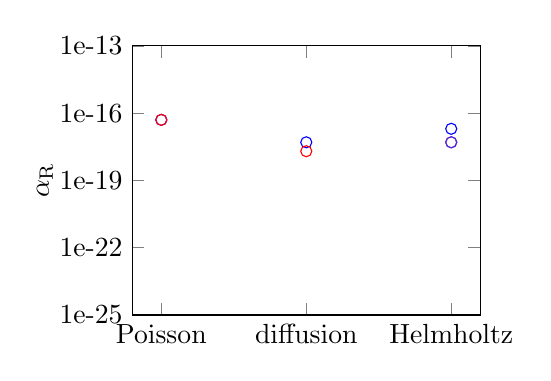
\begin{tikzpicture} 
\begin{axis}
[
    ymode=log,    
    ymin=1e-25,
    ymax=1e-13,
    ytick={1e-25, 1e-22, 1e-19, 1e-16, 1e-13},
    yticklabels={1e-25, 1e-22, 1e-19, 1e-16, 1e-13},   
    legend style={nodes={scale=0.8},at={(0.03,0.85)},anchor=west},
    legend cell align={left},
    height=5cm,
    width=6cm,
    ylabel={$\alpha_{\rm R}$},
    ylabel style={at={(-0.2,0.5)}},    
    xtick={0,1,2,3,4},
    xticklabels={Poisson, diffusion, Helmholtz}
]
\addplot[blue,mark=o, only marks,mark options={color=blue,fill=blue}] coordinates {(0,5.0e-17) (1,5.0e-18) (2,2.0e-17)};
\addplot[red,mark=o, only marks,mark options={color=red,fill=red}] coordinates {(0,5.0e-17) (1,2.0e-18) (2,5.0e-18)};

\addplot[blue,mark=o, only marks,mark options={color=blue!80,fill=blue}] coordinates {(0,5.0e-30) (1,5.0e-30) (2,5.0e-18)};  % SM_Helm_supple
\end{axis}
\end{tikzpicture}}
\caption{First derivative}
\label{alpha_R_Poisson_benchmark_2_diff_2_Helm_grad}
\end{subfigure}
\hspace{-0.7cm}
\begin{subfigure}[b]{0.35\textwidth}
\scalebox{0.85}{
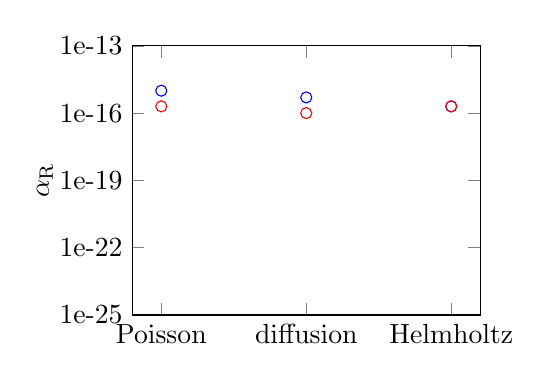
\begin{tikzpicture} 
\begin{axis}
[
    ymode=log,    
    ymin=1e-25,
    ymax=1e-13,
    ytick={1e-25, 1e-22, 1e-19, 1e-16, 1e-13},
    yticklabels={1e-25, 1e-22, 1e-19, 1e-16, 1e-13},     
    legend style={nodes={scale=0.8},at={(0.03,0.85)},anchor=west},
    legend cell align={left},
    height=5cm,
    width=6cm,
    ylabel={$\alpha_{\rm R}$},
    ylabel style={at={(-0.2,0.5)}},    
    xtick={0,1,2,3,4},
    xticklabels={Poisson, diffusion, Helmholtz} 
]
\addplot[blue,mark=o, only marks,mark options={color=blue,fill=blue}] coordinates {(0,1.0e-15) (1,5.0e-16) (2,2.0e-16)};	% SM

\addplot[red,mark=o, only marks,mark options={color=red,fill=red}] coordinates {(0,2.0e-16) (1,1.0e-16) (2,2.0e-16)};		% MM

\end{axis}
\end{tikzpicture}}
\caption{Second derivative}
\label{alpha_R_Poisson_benchmark_2_diff_2_Helm_2ndd}
\end{subfigure}
\caption{Influence of $d(x)$ and $r(x)$ on $\alpha_{\rm R}$ for $p=e^{-(x-0.5)^2}$.}
\label{alpha_R_benchmark_Pois2diff2Helm}
\end{figure}


% \newpage

\bibliographystyle{unsrt}  
\bibliography{mybibfile}  %%% Remove comment to use the external .bib file (using bibtex).


\end{document}
